\documentclass[]{article}
\usepackage{graphicx}
\usepackage{hyperref}
\usepackage[table]{xcolor}
\usepackage{float}
\usepackage[a4paper,bindingoffset=0.2in,%
            left=0.75in,right=0.75in,top=1in,bottom=1in,%
            footskip=.25in]{geometry}
\newcommand{\twolines}[2]{\begin{tabular}{@{}c@{}}#1 \\ #2\end{tabular}}
%opening
\title{Assignment 3 CDA}
\author{Tim van Rossum, 4246306\\
	Michiel Doesburg, 4343875}

\begin{document}

\maketitle

\section{Sampling task}
We ran min-wise sampling on the outgoing IPs of all hosts in the network. The code for this can be found in the script \texttt{sampling.py}, with the data structure for min-wise sampling in the file \texttt{min\_wise\_sample.py}. We also chose to sample from all the hosts instead of only from a few infected hosts, mainly because we did this assignment before it became clear via the Slack channel that you only had to inspect netflows originating from one or several infected hosts. Because we used the same data stream for both the sampling and the sketching task, this does not affect the integrity of the comparison. The table shows the results of min-wise sampling with different reservoir sizes. We chose to use powers of 10 as reservoir sizes as this makes sense with a dataset of roughly 500,000 values. As can be seen from the table, using a reservoir size of 10,000 already reproduces the top 9 correct frequent IP addresses. It makes sense that small the relatively small reservoir sizes of 100 and 1000 make much more approximation errors, since the distribution is approximated by generating a random value for every IP address and storing the lowest k. The bigger the reservoir size the more this will approximate the real distribution. 

\begin{table}[H]
\centering
\caption{Top 10 IP addresses by frequency using min-wise sampling with different reservoir sizes. The real distribution is shown in green. The wrong IPs are shown in red, the right IPs are shown in white.}
\label{my-label}
\resizebox{\columnwidth}{!}{%
\begin{tabular}{|c|c|c|c|c|c|c|c|c|c|c|}
\hline
Reservoir sizes & 1             & 2                                   & 3                                    & 4                                    & 5                                     & 6                                     & 7                                     & 8                                    & 9                                     & 10                                    \\ \hline
\rowcolor[HTML]{A6F499} 
Real data       & \twolines{147.32.84.229}{(60842)} & \twolines{147.32.84.59}{(49223)}                        & \twolines{147.32.80.9}{(47001)}                          & \twolines{147.32.84.138}{(19607)}                       & \twolines{147.32.84.94}{(15489)}                          & \twolines{147.32.80.13}{(5817)}                          & \twolines{147.32.85.7}{(4235)}                           & \twolines{147.32.85.25}{(3242)}                         & \twolines{147.32.85.8}{(3152)}                           & \twolines{147.32.86.134}{(2516)}                         \\ \hline
100             & \twolines{147.32.84.229}{(20)} & \cellcolor[HTML]{FB8282}\twolines{147.32.80.9}{(11)} & \cellcolor[HTML]{FB8282}\twolines{147.32.84.59}{(8)} & \cellcolor[HTML]{FB8282}\twolines{147.32.84.94}{(4)} & \cellcolor[HTML]{FB8282}\twolines{147.32.84.138}{(2)} & \cellcolor[HTML]{FB8282}\twolines{147.32.84.164}{(2)} & \cellcolor[HTML]{FB8282}\twolines{129.241.62.54}{(1)} & \cellcolor[HTML]{FB8282}\twolines{147.32.80.13}{(1)} & \cellcolor[HTML]{FB8282}\twolines{147.32.84.111}{(1)} & \cellcolor[HTML]{FB8282}\twolines{147.32.84.130}{(1)} \\ \hline
1000            & \twolines{147.32.84.229}{(128)} & \cellcolor[HTML]{FB8282}\twolines{147.32.80.9}{(101)} & \cellcolor[HTML]{FB8282}\twolines{147.32.84.59}{(100)} & \twolines{147.32.84.138}{(35)}                        & \twolines{147.32.84.94}{(31)}                          & \twolines{147.32.80.13}{(19)}                          & \twolines{147.32.85.7}{(7)}                           & \cellcolor[HTML]{FB8282}\twolines{147.32.85.8}{(7)}  & \cellcolor[HTML]{FB8282}\twolines{147.32.85.25}{(6)}  & \cellcolor[HTML]{FB8282}\twolines{147.32.85.34}{(5)}  \\ \hline
10000           & \twolines{147.32.84.229}{(1342)} & \twolines{147.32.84.59}{(1125)}                        & \twolines{147.32.80.9}{(985)}                          & \twolines{147.32.84.138}{(432)}                        & \twolines{147.32.84.94}{(349)}                          & \twolines{147.32.80.13}{(132)}                          & \twolines{147.32.85.7}{(97)}                          & \twolines{147.32.85.25}{(75)}                         & \twolines{147.32.85.8}{(61)}                           & \cellcolor[HTML]{FB8282}\twolines{88.176.79.163}{(60)} \\ \hline
100000          & \twolines{147.32.84.229}{(13220)} & \twolines{147.32.84.59}{(10798)}                        & \twolines{147.32.80.9}{(10432)}                          & \twolines{147.32.84.138}{(4346)}                        & \twolines{147.32.84.94}{(3359)}                          & \twolines{147.32.80.13}{(1264)}                          & \twolines{147.32.85.7}{(912)}                           & \twolines{147.32.85.25}{(716)}                         & \twolines{147.32.85.8}{(687)}                           & \cellcolor[HTML]{FB8282}\twolines{88.176.79.163}{(606)} \\ \hline
\end{tabular}
}
\end{table}
\section{Sketching task}

We also performed count-min sketching to estimate the distribution of data in the stream. The code for this can be found in the \texttt{sketching.py} file. This code uses an implementation of the count-min sketch data structure that we got from \url{https://github.com/rafacarrascosa/countminsketch}. The code for this can be found in the file \texttt{count\_min\_sketch.py}. The code has been adapted to work with Python 3 as we use this for our assignment. Table 2 shows the top ten most frequently occurring IP addresses when sampling is performed with different amounts of hash functions and different table sizes, compared to the actual top ten. Once again, we decided to include all hosts in the sample, also mainly due to the fact that we did this before it was clear via Slack that only some infected hosts needed to be sampled. Another reason was to keep the hosts of which we sample netflows consistent to allow for comparison of sampling methods. The error is determined by the values for $w$ (table depth) and $d$ (amount of hash functions). Where $\epsilon = e/w$ and $\delta = e^{-d}$. At $w=10$ and $d=10$, we get $\epsilon = 0.27$ and $1 - \delta = 0.9996$ Meaning the results are within an additive error of 0.27 with 0.9996 probability. At $w = 100$ and $d = 30$, these values are already at $\epsilon = 0.03$ and $\delta = 0.999999$. We can see from the table that indeed for these values the algorithm performs very well.
Comparing the space requirements, the sampling algorithm works well for a reservoir size of 10,000. The sketching algorithm already performs better for a matrix of size 100x10 = 1000 cells. Without performing an in-depth comparison, it seems that the sketching algorithm is much more space efficient, and also much more accurate with the same space allotment. As such, we would recommend count-min sketching for estimating the distribution of stream data.


\begin{table}[H]
\centering
\caption{The top 10 IP addresses by frequency using Count-Min sketching with different amount of hash functions and table depths.}
\label{my-label}
\resizebox{\columnwidth}{!}{%
\begin{tabular}{|c|c|c|c|c|c|c|c|c|c|c|c|}
\hline
table size              & \# hash functions             & 1                                                          & 2                                     & 3                                      & 4                                    & 5                                       & 6                                   & 7                                     & 8                                     & 9                                      & 10                                      \\ \hline
\rowcolor[HTML]{A6F499} 
\multicolumn{2}{|l|}{\cellcolor[HTML]{A6F499}Real data} & \twolines{147.32.84.229}{(60842)} & \twolines{147.32.84.59}{(49223)}                        & \twolines{147.32.80.9}{(47001)}                          & \twolines{147.32.84.138}{(19607)}                       & \twolines{147.32.84.94}{(15489)}                          & \twolines{147.32.80.13}{(5817)}                          & \twolines{147.32.85.7}{(4235)}                           & \twolines{147.32.85.25}{(3242)}                         & \twolines{147.32.85.8}{(3152)}                           & \twolines{147.32.86.134}{(2516)}   \\ \hline
10                      & 10                            & \twolines{147.32.84.229}{(82640)}                                              & \twolines{147.32.84.59}{(70845)} & \twolines{147.32.80.9}{(66909)} & \cellcolor[HTML]{FB8282}\twolines{219.110.226.187}{(51078)} & \cellcolor[HTML]{FB8282}\twolines{194.192.199.252}{(45538)} & \cellcolor[HTML]{FB8282}\twolines{147.32.80.9}{(39213)} & \cellcolor[HTML]{FB8282}\twolines{94.240.131.96}{(37850)} & \cellcolor[HTML]{FB8282}\twolines{77.247.23.118}{(36529)} & \cellcolor[HTML]{FB8282}\twolines{114.89.216.15}{(36529)}  & \cellcolor[HTML]{FB8282}\twolines{80.130.223.250}{(36529)}  \\ \hline
10                      & 20                            & \twolines{147.32.84.229}{(81855)}                                              & \twolines{147.32.84.59}{(66795)}                          & \twolines{147.32.80.9}{(65935)}                            & \twolines{147.32.84.138}{(40895)}                        & \twolines{147.32.84.94}{(38368)}                            & \cellcolor[HTML]{FB8282}\twolines{93.65.50.92}{(28902)} & \cellcolor[HTML]{FB8282}\twolines{89.28.60.71}{(28116)}   & \twolines{147.32.85.25}{(28116)}                          & \cellcolor[HTML]{FB8282}\twolines{111.252.83.165}{(27872)} & \cellcolor[HTML]{FB8282}\twolines{213.146.167.107}{(27872)} \\ \hline
10                      & 30                            & \twolines{147.32.84.229}{(81778)}                                              & \twolines{147.32.84.59}{(69850)}                          & \twolines{147.32.80.9}{(67986)}                            & \twolines{147.32.84.138}{(39646)}                        & \twolines{147.32.84.94}{(36578)}                            & \twolines{147.32.80.13}{(28640)}                        & \cellcolor[HTML]{FB8282}\twolines{93.36.215.109}{(28447)} & \cellcolor[HTML]{FB8282}\twolines{147.32.85.26}{(27948)}  & \cellcolor[HTML]{FB8282}\twolines{78.8.100.201}{(27948)}   & \cellcolor[HTML]{FB8282}\twolines{147.32.192.127}{(27948)}  \\ \hline
100                     & 10                            & \twolines{147.32.84.229}{(61957)}                                              & \twolines{147.32.84.59}{(50599)}                          & \twolines{147.32.80.9}{(48086)}                            & \twolines{147.32.84.138}{(21083)}                        & \twolines{147.32.84.94}{(17023)}                            & \twolines{147.32.80.13}{(6971)}                        & \twolines{147.32.85.7}{(5548)}                           & \twolines{147.32.85.25}{(4680)}                          & \twolines{147.32.85.8}{(4404)}                            & \twolines{147.32.86.134}{(4338)}                           \\ \hline
100                     & 20                            & \twolines{147.32.84.229}{(62271)}                                              & \twolines{147.32.84.59}{(50660)}                          & \twolines{147.32.80.9}{(48232)}                            & \twolines{147.32.84.138}{(21087)}                        & \twolines{147.32.84.94}{(17142)}                            & \twolines{147.32.80.13}{(7421)}                        & \twolines{147.32.85.7}{(5673)}                           & \twolines{147.32.85.25}{(4721)}                          & \twolines{147.32.85.8}{(4538)}                            & \twolines{147.32.86.134}{(4001)}                           \\ \hline
100                     & 30                            & \twolines{147.32.84.229}{(62290)}                                              & \twolines{147.32.84.59}{(50521)}                          & \twolines{147.32.80.9}{(48515)}                            & \twolines{147.32.84.138}{(21029)}                        & \twolines{147.32.84.94}{(16834)}                            & \twolines{147.32.80.13}{(7065)}                        & \twolines{147.32.85.7}{(5883)}                           & \twolines{147.32.85.25}{(4345)}                          & \twolines{147.32.85.8}{(4339)}                            & \cellcolor[HTML]{FB8282}\twolines{88.176.79.163}{(3779)}   \\ \hline
1000                    & 10                            & \twolines{147.32.84.229}{(60897)}                                              & \twolines{147.32.84.59}{(49287)}                          & \twolines{147.32.80.9}{(47082)}                            & \twolines{147.32.84.138}{(19687)}                        & \twolines{147.32.84.94}{(15566)}                            & \twolines{147.32.80.13}{(5903)}                        & \twolines{147.32.85.7}{(4294)}                           & \twolines{147.32.85.25}{(3299)}                          & \twolines{147.32.85.8}{(3209)}                            & \twolines{147.32.86.134}{(2584)}                           \\ \hline
1000                    & 20                            & \twolines{147.32.84.229}{(60892)}                                              & \twolines{147.32.84.59}{(49286)}                          & \twolines{147.32.80.9}{(47055)}                            & \twolines{147.32.84.138}{(19674)}                        & \twolines{147.32.84.94}{(15554)}                            & \twolines{147.32.80.13}{(5867)}                        & \twolines{147.32.85.7}{(4280)}                           & \twolines{147.32.85.25}{(3298)}                          & \twolines{147.32.85.8}{(3230)}                            & \twolines{147.32.86.134}{(2573)}                           \\ \hline
1000                    & 30                            & \twolines{147.32.84.229}{(60896)}                                              & \twolines{147.32.84.59}{(49278)}                          & \twolines{147.32.80.9}{(47050)}                            & \twolines{147.32.84.138}{(19654)}                        & \twolines{147.32.84.94}{(15543)}                            & \twolines{147.32.80.13}{(5877)}                        & \twolines{147.32.85.7}{(4290)}                           & \twolines{147.32.85.25}{(3302)}                          & \twolines{147.32.85.8}{(3223)}                            & \twolines{147.32.86.134}{(2599)}                           \\ \hline
10000                   & 10                            & \twolines{147.32.84.229}{(60842)}                                              & \twolines{147.32.84.59}{(49226)}                       & \twolines{147.32.80.9}{(47001)}                            & \twolines{147.32.84.138}{(19608)}                        & \twolines{147.32.84.94}{(15490)}                            & \twolines{147.32.80.13}{(5820)}                        & \twolines{147.32.85.7}{(4238)}                           & \twolines{147.32.85.25}{(3245)}                          & \twolines{147.32.85.8}{(3156)}                            & \twolines{147.32.86.134}{(2518)}                           \\ \hline
10000                   & 20                            & \twolines{147.32.84.229}{(60842)}                                              & \twolines{147.32.84.59}{(49223)}                           & \twolines{147.32.80.9}{(47001)}                            & \twolines{147.32.84.138}{(19608)}                        & \twolines{147.32.84.94}{(15490)}                            & \twolines{147.32.80.13}{(5820)}                        & \twolines{147.32.85.7}{(4238)}                           & \twolines{147.32.85.25}{(3245)}                          & \twolines{147.32.85.8}{(3156)}                            & \twolines{147.32.86.134}{(2518)}                           \\ \hline
10000                   & 30                            & \twolines{147.32.84.229}{(60842)}                                              & \twolines{147.32.84.59}{(49224)}                           & \twolines{147.32.80.9}{(47001)}                            & \twolines{147.32.84.138}{(19608)}                        & \twolines{147.32.84.94}{(15490)}                            & \twolines{147.32.80.13}{(5820)}                        & \twolines{147.32.85.7}{(4238)}                           & \twolines{147.32.85.25}{(3245)}                          & \twolines{147.32.85.8}{(3156)}                            & \twolines{147.32.86.134}{(2518)}                           \\ \hline
\end{tabular}
}
\end{table}
\section{Botnet flow data discretization task}
Before we could begin on this task, we first had to know which two features to use and to discretize. To that end, we made visualizations. As can be seen in figure~\ref{protocol}, the protocol used in a netflow provides a very strong predictor for maliciousness. Almost all botnet netflows use the ICMP protocol in Scenario 10. in figure~\ref{flags}, it can also be seen that the botnet netflows generally use the flags ECO or ECR, while legitimate netflows use different flags. As such, these two features are very discriminatory, and we decided to use these features in the discretization task. The discretization is applied in the script \texttt{discretization.py}. Behaviour we observe in the two features that could be useful for detecting the infection with a sequential model is that clearly a machine producing several ICMP netflows is very likely to be malicious. As such, we decided to use these two features for the discretization of the netflows. These features are kept, and the netflows are then transformed to a single value based on the method in paper 4. These values will then be discretized using SAX. Every transformed netflow will be represented by a single letter, as to not skip over any netflows that might be useful.
\begin{figure}[H]
\begin{center}
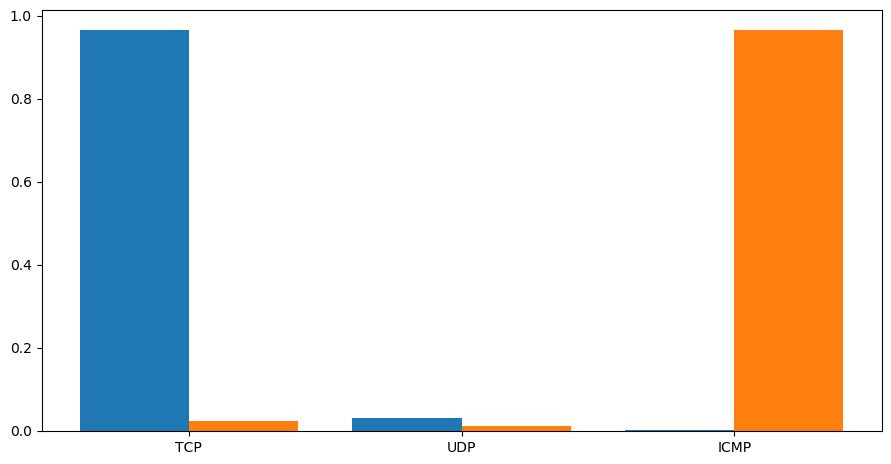
\includegraphics[scale=0.4]{scenario10_networkprotocol.png}
\caption{Percentage of netflows per network protocol. Benign netflows are shown in blue, malicious netflows are in orange. Nearly all malicious netflows use the ICMP protocol, while nearly all benign netflows use TCP. }
\label{protocol}
\end{center}
\end{figure}
\begin{figure}[H]
\begin{center}
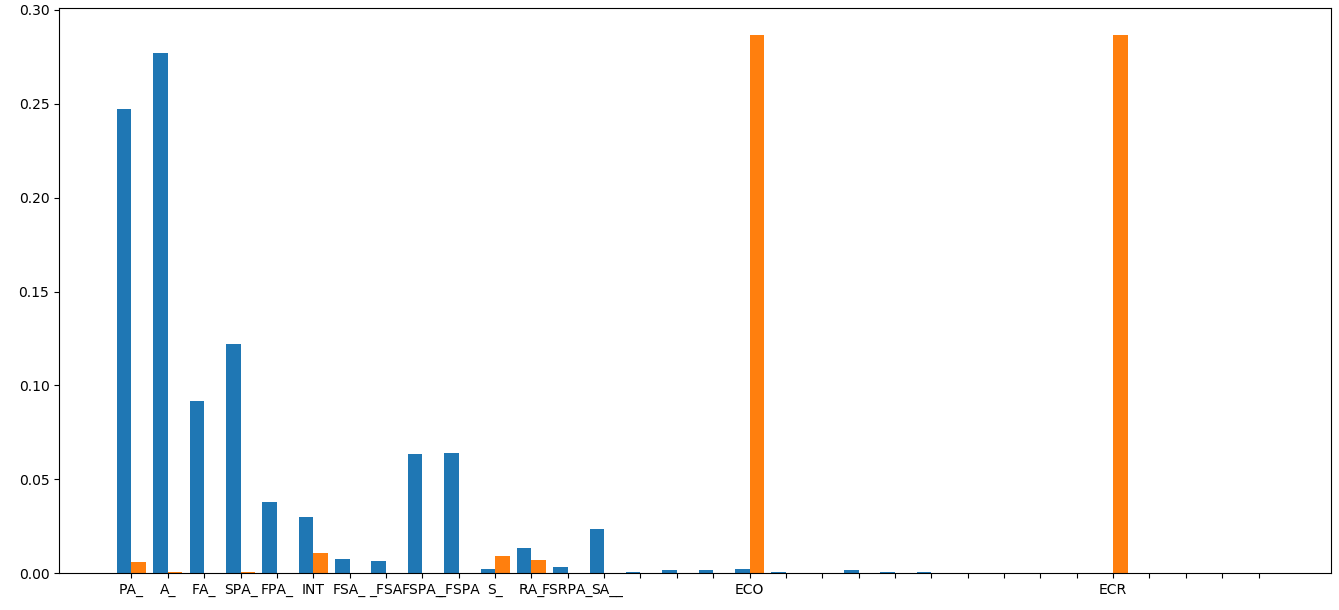
\includegraphics[scale=0.4]{scenario10_flags.png}
\caption{Percentage of netflows per flag type. Benign netflows are shown in blue, malicious netflows are in orange. The flags `ECO' and `ECR' account for nearly 60\% of all malicious netflows.}
\label{flags}
\end{center}
\end{figure}
\section{Botnet profiling task}
For our sequential data mining model, we decided to use Ngrams. We worked as follows: we would determine the discretized netflow of a host for every host in the dataset. Then, we would select one discretized netflow from an infected host, and one discretized netflow from a non-infected host. A host is deemed infected if at least one netflow originating from that host is a botnet netflow. The discretized netflows that we select as examples are selected randomly. Then, for all the discretized netflows, we would compare the discretized netflows with our two examples. If the new discretized netflow looked more like the profile of a non-infected host, then the host was deemed as not infected, and if it looked more like the profile of an infected host, then the host was classified as infected. This way of working gave the following results:
\begin{itemize}
	\item TP: 46
    \item FP: 345
    \item TN: 110
    \item FN: 21
\end{itemize}
The false positive rate for this technique is high, but the amount of true and false positives depend heavily on which host is selected. Instead of randomly selecting examples, we tried a different approach and selected the longest discretized netflow for both a infected host and a non-infected host. This gave the following results:
\begin{itemize}
	\item TP: 13
    \item FP: 1
    \item TN: 454
    \item FN: 54
\end{itemize}
As can be seen, the amount of successful detections has gone down a lot, but the false positive rate has also dropped. In general in the field of threat detection, it is better to miss cases where there is anomalous behaviour to get less false positives, as every single false positive warrants an unnecessary investigation. Therefore, the approach of using the longest discretized netflow is better in our opinion. It should also be noted that one true positive and one true negative from both cases comes from the examples for an infected host and a non-infected host being used to check whether or not the host is infected, skewing the results somewhat, but not by a lot.
\section{Bonus task}
As explained in section about botnet netflow discretization, the flags of a netflow and the protocol of a netflow are very discriminative information in Scenario 10. Because of this, we though that we could use these features to classify netflows to be botnet netflows or legitimate netflows. To this end, we used only these two features, transformed them using the label encoded included in sklearn to transform them to numerical values, and classified them using 10-fold cross validation with a standard linear classifier with no changed parameters whatsoever, just to test how good classification could be. We did not apply SMOTE to the dataset to balance out malicious and benign netflows, as the total amount of malicious netflows and the total amount of benign netflows differed less than 1000 of each other, making SMOTE not really that useful as the classes are already balanced to less than 1\% difference in the amount of datapoints per class. On the packet level, every netflow was treated as a single datapoint. This gave the following results:
\begin{itemize}
	\item TP: 311045
    \item FP: 1014
    \item TN: 320903
	\item FN: 11113
\end{itemize}
As can be seen, the performance is really good using just these two features, no SMOTE (because it is not necessary here) and no further optimization of the classifier.

For host-based classification, we first looked at the amount of infected hosts versus the amount of non-infected hosts. A host was deemed infected if at least one netflow originating from that host was classified as a botnet netflow. There were more than 500 different hosts, of which less than 70 were infected. Because the amount of botnet netflows and legitimate netflows is roughly the same, it is reasonable to think that the average infected host has a lot more netflows going out of it compared to the average non-infected host. As such, we decided to use the amount of netflows that originated from a single host as the feature of a host to decide whether or not it is an infected host. We did perform SMOTE on the training data here, as there were more than 500 different hosts, of which less than 70 were infected. We again used standard linear regression and 10-fold cross validation, and got the following results:
\begin{itemize}
	\item TP: 12
    \item FP: 23
    \item TN: 432
	\item FN: 55
\end{itemize}
This result is worse than netflow-based classification and host-based classification using ngrams to search for string similarity, but still rather good. The performance of the netflow-based classification, however, is a definite winner in our opinion over all the other methods, as the features selected are extremely discriminatory. As such, in this case, we prefer using a classifier over a sequential model.
\section{Link to our Github repo}
All code can be found on \url{https://github.com/Michieldoesburg/cyber_data_analytics}. The code for this assignment is, of course, in the \texttt{assignment3} folder.
\bibliography{bibliography}
\bibliographystyle{unsrt}
\end{document}
